% ROB-Newguide.tex
% v1.1, released 25 Feb 2021
% Copyright 2021 Cambridge University Press

\documentclass[DTMColor]{ROB-New}

\begin{document}

\authormark{Cambridge Authors}

\articletype{RESEARCH ARTICLE}

\jnlPage{1}{7}
\jyear{2021}
\jdoi{10.1017/xxxxx}

\title{Robotica: \LaTeX Guidelines for~authors}

\author[1]{First Author\hyperlink{corr}{*}}
\address[1]{Affiliation 1, Country}

\author[2]{ Second Author}
\address[2]{Affiliation 2, Country}
\address{\hypertarget{corr}{*}Corresponding author. \email{email address}}

\received{xx xxx xxx}
\revised{xx xxx xxx}
\accepted{xx xxx xxx}

\keywords{keyword1, keyword2}

\abstract{This guide is for authors who are preparing papers for the {\em Robotica} journal using the \LaTeX\ document preparation system and the CUP ROB style file.}

\maketitle

\section{Introduction}

The layout design for the {\em Robotica} journal
has been implemented as a \LaTeX\ style file. The ROB style file is based
on the ARTICLE style as discussed in the \LaTeX\ manual. Commands which
differ from the standard \LaTeX\ interface, or which are provided in addition
to the standard interface, are explained in this guide. This guide is not a
substitute for the \LaTeX\ manual itself.

\subsection{Introduction to \LaTeX}

The \LaTeX\footnote{To know more information about LaTeX and its packages, try https://ctan.org/?lang=en}\ document preparation system is a special version of the
\TeX\ typesetting program. \LaTeX\ adds to \TeX\ a collection of
commands which simplify typesetting by allowing the author to
concentrate on the logical structure of the document rather than
its visual layout.

\LaTeX\ provides a consistent and comprehensive document preparation
interface. There are simple-to-use commands for generating a table of
contents, lists of figures and/or tables, and indexes. \LaTeX\ can
automatically number list entries, equations, figures, tables, and
footnotes, as well as parts, chapters, sections and subsections.
Using this numbering system, bibliographic citations, page references
and cross references to any other numbered entity ({\it e.g.\ } chapter,
section, equation, figure, list entry) are quite straightforward.

\subsection{The ROB document class}

The use of document class allows a simple change of style (or style option like if DTMColor is removed from \verb"\documentclass" then the layout will be in B/W)
to transform the appearance of your document. The CUP ROB class file preserves
the standard \LaTeX\ interface such that any document which can be produced
using the standard \LaTeX\ ARTICLE style can also be produced with the
ROB style. However, the fonts (sizes) and measure of text is slightly different
from that for ARTICLE, therefore line breaks will change and it is possible
that equations may need re-setting.

\section{Additional facilities}

In addition to all the standard \LaTeX\ design elements, the ROB style
includes the following feature:
\begin{itemize}
  \item Extended commands for specifying a short version
        of the title and author(s) for the running
        headlines.
\end{itemize}
Once you have used this additional facility in your document,
do not process it with a standard \LaTeX\ style file.

\subsection{Titles authors' names and affiliation}

In the ROB style, the title of the article and the author's name (or authors'
names) are used both at the beginning of the article for the main title and
throughout the article as running headlines at the top of every page.
The title is used on odd-numbered pages (rectos) and the author's name appears
on even-numbered pages (versos).
Although the main heading can run to several lines of text, the running head
line must be a single line.

Moreover, the main heading can also incorporate new line commands
({\it e.g.\ } \verb"\\") but these are not acceptable in a running headline.
To enable you to specify an alternative short title and author's name, the
standard \verb"\authormark" command have been used to print the author running headline. If more authors has to be used in \verb"\author" command then each authors should be captured in separate \verb"\author" command.
\verb"\address" command is used to call the affiliation, if more affiliations has to be used in \verb"\address" command then each affiliations should be captured in separate \verb"\address" command. The author and affiliation indicator should be catptured with an option argument in \verb"\author" and \verb"\address" command such as \verb"\author[..]" and \verb"\address[..]". The \verb"\email" command should be used inside the affiliation:
%
\begin{verbatim}
  \authormark{Cambridge Authors}
  \title{The full title which can be as long as necessary}
  \author{Author's name}
  \address{the affiliation if necessary\email{email}}
\end{verbatim}
%
\subsection{Abstract}

The ROB style provides for an abstract which is produced by the following
commands
%
\begin{verbatim}
  \begin{abstract}  ...  \end{abstract}
\end{verbatim}

\subsection{Lists}

The ROB style provides the three standard list environments.
\begin{itemize}
  \item Bulleted lists, created using the \verb"itemize" environment.
  \item Numbered lists, created using the \verb"enumerate" environment.
  \item Labelled lists, created using the \verb"description" environment.
\end{itemize}

\subsection{Footnotes}

The ROB journal style uses superior numbers for footnote
references.\footnote{This shows how a footnote is typeset.}

\section{Some guidelines for using standard facilities}

The following notes may help you achieve the best effects with the ROB style
file.

\subsection{Sections}

\LaTeX\ provides five levels of section headings and they are all
defined in the ROB style file:
\begin{itemize}
  \item \verb"\section".
  \item \verb"\subsection".
  \item \verb"\subsubsection".
  \item \verb"\paragraph".
  \item \verb"\subparagraph".
\end{itemize}
Section numbers are given for sections, subsection and subsubsection headings.

\subsection{Running headlines}

As described above, the author's name (or author's
names) should be used as running headline at the top of every page.
The journal title is used on odd-numbered pages (rectos) and the author's name appears
on even-numbered pages (versos).

The \verb"\pagestyle" and \verb"\thispagestyle" commands should {\em not\/} be
used.
Similarly, the commands \verb"\markright" and \verb"\markboth" should not be
necessary.


\subsection{Tables}

The {\tt figure} and {\tt table} environments are implemented as described in
the \LaTeX\ Manual to
provide consecutively numbered floating inserts for illustrations and tables
respectively.
The standard inserts and their captions are formatted centred.
Line breaks in captions can be inserted as required using \verb"\\".

The ROB style file will cope with most positioning of your tables
and you should not normally use the optional positional qualifiers on the
\verb"table" environment which would override these decisions.
Normal journal style sets the table caption first, followed by a double
rule, the table body and a double rule at the bottom.  Single rules and
spanner rules (\verb"\cline") can be used to separate headings from the
columns.  For example, Table~\ref{sample-table} is produced using the
following commands:\vskip0pt
%
{\fontsize{7}{9}\selectfont
\begin{verbatim}
\begin{table}
  \TBL{\caption{Results of Overloading for 3 Experimental Setups\label{sample-table}}}
  {\begin{fntable}\centering
    \begin{tabular}{@{\extracolsep{\fill}}lcrrrrr}
    \hline
    Program& Expt.&CPU&RelCPU&GC& Mem&RelMem\\
    \hline
    8 Queens& (a)&   2 88&  1 00&    6&   1 7M&  1 00\\
    &         (b)&  32 51& 11 29&  193&  48 9M& 28 76\\
    &         (c)&   7 90&  2 74&   42&  11 3M&  6 65\\
    Primes&   (a)&   4 89&  1 00&   19&   5 3M&  1 00\\
    &         (b)&  47 54&  9 72&  204&  54 5M& 10 28\\
    &         (c)&  10 08&  2 06&   47&  13 0M&  2 45\\
    Nfib&     (a)&  21 65&  1 00&  161&  40 4M&  1 00\\
    &         (b)& 221 65& 10 24& 1382& 349 0M&  8 64\\
    &         (c)&  21 30&  0 98&  161&  42 0M&  1 03\\
    \hline
    \end{tabular}
  \end{fntable}}
\end{table}
\end{verbatim}}
%
\noindent Notice the use of the \verb"" macro to obtain the centered
decimal points, inside the body of the table.

\begin{table}[h!]
  \TBL{\caption{Results of Overloading for 3 Experimental Setups\label{sample-table}}}
 {\begin{fntable}\centering
    \begin{tabular}{@{\extracolsep{\fill}}lcrrrrr}
    \hline
     Program& Expt.&CPU&RelCPU&GC& Mem&RelMem\\
    \hline
    8 Queens& (a)&   2 88&  1 00&    6&   1 7M&  1 00\\
    &         (b)&  32 51& 11 29&  193&  48 9M& 28 76\\
    &         (c)&   7 90&  2 74&   42&  11 3M&  6 65\\
    Primes&   (a)&   4 89&  1 00&   19&   5 3M&  1 00\\
    &         (b)&  47 54&  9 72&  204&  54 5M& 10 28\\
    &         (c)&  10 08&  2 06&   47&  13 0M&  2 45\\
    Nfib&     (a)&  21 65&  1 00&  161&  40 4M&  1 00\\
    &         (b)& 221 65& 10 24& 1382& 349 0M&  8 64\\
    &         (c)&  21 30&  0 98&  161&  42 0M&  1 03\\
    \hline
    \end{tabular}
  \end{fntable}}
\end{table}

The \verb"tabular" environment should be used to produce ruled tables;
it has been modified for the ROB style in the following ways:
\begin{enumerate}
  \item Additional vertical space is inserted above and below a horizontal rule
        (produced by \verb"\hline");
\end{enumerate}
Because of this reformatting, vertical rules should not be used;
furthermore, commands to
redefine quantities such as \verb"\arraystretch" should be omitted. If
the old tabular facilities are needed, there is a new environment,
\verb"oldtabular", which has none of the reformatting; it should be used
in exactly the same way.

\subsection{Illustrations (or figures)}

The ROB style will cope with most positioning of your illustrations
and you should not normally use the optional positional qualifiers on
the \verb"figure" environment which would override these decisions.
Figure captions should be below the figure itself, therefore the \verb"\caption"
command should appear after the figure or space left for an illustration.
Figure~\ref{sample-figure} shows an example of working with LaTeX code, where the \verb"\includegraphics" command is used to load art files. The \verb"scale" option is used in \verb"\includegraphics" to reduce the size of the image. EPS format will be compiled using LaTeX. PNG, PDF and JPG format art files are loaded in the same command but the TeX file should be compiled using PDFLaTeX:
%
\begin{verbatim}
  \begin{figure}
    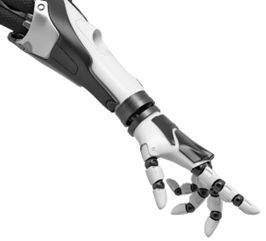
\includegraphics[scale=.4]{sample.eps}
    \caption{An example figure with space for artwork}
    \label{sample-figure}
  \end{figure}
\end{verbatim}
%
The vertical depth should correspond roughly to the artwork you will submit;
it will be adjusted to fit the final artwork exactly.
%
\begin{figure}[hbt!]
  \centerline{\vbox to 6pc{\hbox to 10pc{}}}
  %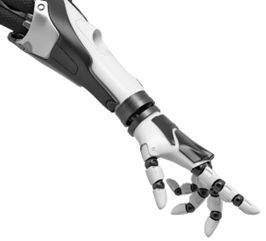
\includegraphics[scale=.4]{sample.eps}
  \caption{An example figure with space for artwork}
  \label{sample-figure}
\end{figure}
%
\subsection{Creating new theorem-like environments}

You can create your own environments in \LaTeX, and although you may already
be familiar with \verb"\newtheorem", you will not have seen the other two
commands explained below.

\verb"\newtheorem" is a standard command used for creating new
        theorem-like environments, such as theorems, corollaries, lemmas,
        conjectures and propositions, with the body of the text
        (automatically) in italic.

\section{Mathematics}

The ROB class file will centre displayed mathematics, and will insert the
correct space above and below if standard \LaTeX\ commands are used; for
example use \verb"\[ ... \]" and \emph{not} \verb"$$ ... $$". Do not leave
blank lines above and below displayed equations unless a new paragraph is
really intended.

\verb"amsmath.sty" is common package to handle various type math equations. The amsmath descriptions are available in the document can be find in the web link \verb"https://ctan.org/pkg/amsmath?lang=en"

\subsection{Numbering of equations}

The \verb"subequations" and \verb"subeqnarray" environments have been
incorporated into the ROB class file (see Section~\ref{sub:amstex} regarding
the \verb"subequations" environment). Using these two environments,
you can number your equations (\ref{a1}), (\ref{a2}) etc. automatically.
For example, you can typeset
  \begin{subequations}
  \begin{equation}
    a_1 \equiv (2\Omega M^2/x)^{\textstyle\frac{1}{4}}
      y^{\textstyle\frac{1}{2}}\label{a1}
  \end{equation}
  and
  \begin{equation}
    a_2 \equiv (x/2\Omega)^{\textstyle\frac{1}{2}}k_y/M.\label{a2}
  \end{equation}
  \end{subequations}
by using the \verb"subequations" environment as follows:
%
\begin{verbatim}
  \begin{subequations}
  \begin{equation}
    a_1 \equiv (2\Omega M^2/x)^{\textstyle\frac{1}{4}}
      y^{\textstyle\frac{1}{2}}\label{a1}
  \end{equation}
  and
  \begin{equation}
    a_2 \equiv (x/2\Omega)^{\textstyle\frac{1}{2}}k_y/M.\label{a2}
  \end{equation}
  \end{subequations}
\end{verbatim}

\subsubsection{The \texttt{subequations} environment and the
  \texttt{AMSTEX} package} \label{sub:amstex}

The \verb"amstex" (and the \verb"amsmath") packages also define a
\verb"subequations" environment.  The environment in \verb"ROB.cls" is used
by default, as the environments in the AMS packages don't produce the correct
style of output.

Note that the \verb"subequations" environment from the \verb"amstex" package
takes an argument -- you should use an `a' to give \verb"\alph" style
subequations. e.g.
\begin{verbatim}
  \begin{subequations}{a}  ...  \end{subequations}
\end{verbatim}

\subsection{Bibliography}

As with standard LaTeX, there are two ways of producing a bibliography;
either by compiling a list of references by hand (using a
\verb"thebibliography" environment), or by using BibTeX with a suitable
bibliographic database for example sample.bib with the bibliography style provided with the ROB-New-Guide.tex like \verb"\bibliographystyle{roblike}". The roblike.bst will produce the bibliography which is similar to rob style but not exactly. If any modification has to be made with roblike.bst can be adjusted during manuscript preparation but the updated bst file should be given with source files. However, contributors are encouraged to format their list of references style outlined in section~\ref{fullref} below.

\subsubsection{References in the text}

References in the text are given by reference number.
Whichever method is used to produce the bibliography, the references in
the text are done in the same way. Each bibliographical entry has a key,
which is assigned by the author and used to refer to that entry in the
text. There is one form of citation -- \verb"\cite{key}" -- to produce the
reference number. Thus, \cite{JOE.2000} is produced~by
\begin{verbatim}
  \cite{JOE.2000}.
\end{verbatim}

\verb"natbib.sty" is common package to handle various reference and its cross citations. The natbib descriptions are available in the document can be find in the web link \verb"https://ctan.org/pkg/natbib?lang=en"

\subsubsection{List of references}\label{fullref}

The following listing shows some references prepared in the style of the
journal.
%
{\fontsize{7}{9}\selectfont
\begin{verbatim}
\begin{thebibliography}{99}
\bibitem{Antonelli-SpingerBook2013}
G. Antonelli, {\it Underwater Robots}, vol. 96. Springer Tracts in Advanced
Robotics (Springer International Publishing, Switzerland, 2014).
\bibitem{Fossen2011handbook}
T. I. Fossen, {\it Handbook of Marine Craft Hydrodynamics and Motion Control}
(John Wiley \& Sons, Ltd., United Kingdom, 2011).
\bibitem{deBarros_JOE2019}
P. Cardenas and E. A. de Barros, ``Estimation of AUV hydrodynamic coefficients
using analytical and system identification approaches,'' {\it IEEE J. Ocean.
Eng.}, 1--20 (2019). 10.1109/JOE.2019.2930421
\bibitem{JOE.2000}
M. Caccia, G. Indiveri and G. Veruggio, ``Modelling and identification of
open-frame variable configuration unmanned underwater vehicles,'' {\it IEEE J.
Ocean. Eng.} \textbf{5}, 227--240 (2000).
\bibitem{peng2018path}
Z. Peng, J. Wang and Q.-L. Han, ``Path-following control of autonomous underwater
vehicles subject to velocity and input constraints via neurodynamic optimization,''
{\it IEEE Trans. Ind. Electron.} \textbf{66}(11), 8724--8732 (2018).
\end{thebibliography}
\end{verbatim}}
%
\subsection{Catchline and date commands}

To be placed in the preamble; for example:

\begin{itemize}
  \item \verb"\jyear{2021}"
  \item \verb"\jdoi{10.1017/xxxxx}"
  \item \verb"\jnlPage{1}{8}"
  \item \verb"\received{xx xxx xxx}\revised{xx xxx xxx}\accepted{xx xxx xxx}"
\end{itemize}

\begin{con}
\ctitle{Author Contributions}
A short statement must be provided indicating how each author contributed to the work. For example: AB and CD conceived and designed the study. CD and EF conducted data gathering. GH performed statistical analyses. AB, EF and GH wrote the article.

\ctitle{Financial Support}
If you have nothing to declare, write This research received no specific grant from any funding agency, commercial or not-for-profit sectors.

\ctitle{Conflicts of Interest}
You must declare any potential conflicts of interest, whether personal, financial or other. If there is nothing, write The authors declare no conflicts of interest exist.

\ctitle{Ethical Approval}
If your paper includes experimentation with vertebrates, you must give details here of the body that approved the study, together with any relevant identification number. If your study did not include such experiments, write Not applicable.

\ctitle{Acknowledgements}
You may also include an Acknowledgements section if you wish. Please note that this must be separate from the Financial Support declaration.
\textbf{Please note: If you have used AI in the research or preparation of the manuscript, this MUST be declared in the Acknowledgements. Authors should state what tool was used, what it was used for, and confirm that all authors reviewed the content and take full responsibility for the paper.}
\end{con}
%
\vspace{5mm} %5mm vertical space

[The following reference list is for illustration purposes only]
\begin{thebibliography}
{99}
\bibitem{Antonelli-SpingerBook2013}
G. Antonelli, {\it Underwater Robots}, vol. 96. Springer Tracts in Advanced Robotics (Springer International Publishing, Switzerland, 2014).
\bibitem{Fossen2011handbook}
T. I. Fossen, {\it Handbook of Marine Craft Hydrodynamics and Motion Control} (John Wiley \& Sons, Ltd., United Kingdom, 2011).
\bibitem{deBarros_JOE2019}
P. Cardenas and E. A. de Barros, ``Estimation of AUV hydrodynamic coefficients using analytical and system identification approaches,'' {\it IEEE J. Ocean. Eng.}, 1--20 (2019). 10.1109/JOE.2019.2930421
\bibitem{JOE.2000}
M. Caccia, G. Indiveri and G. Veruggio, ``Modelling and identification of open-frame variable configuration unmanned underwater vehicles,'' {\it IEEE J. Ocean. Eng.} \textbf{5}, 227--240 (2000).
\bibitem{peng2018path}
Z. Peng, J. Wang and Q.-L. Han, ``Path-following control of autonomous underwater vehicles subject to velocity and input constraints via neurodynamic optimization,'' {\it IEEE Trans. Ind. Electron.} \textbf{66}(11), 8724--8732 (2018).
\end{thebibliography}

\end{document}
